\documentclass[14pt,a4paper]{extarticle}
\usepackage{iftex}
\ifXeTeX
\usepackage{fontspec}
\defaultfontfeatures{Ligatures=TeX}
\setmainfont{Times New Roman}
\setmonofont{DejaVu Sans Mono}
\else
\usepackage[T2A]{fontenc}
\usepackage[utf8]{inputenc}
\fi
\usepackage[russian]{babel}
\usepackage[top=20mm, bottom=20mm, left=30mm, right=15mm]{geometry}
\usepackage{setspace}
\usepackage{indentfirst}
\usepackage{titlesec}
\usepackage{graphicx}
\graphicspath{{images/}{../report/}}
\usepackage{amsmath}
\usepackage{caption}
\usepackage{microtype}
\usepackage{listings}
\usepackage{placeins}
\usepackage{verbatim}
\usepackage{amssymb}

\makeatletter
\def\verbatim@font{\ttfamily\footnotesize}
\makeatother

\usepackage[
    pdftitle={Отчёт по преддипломной практике},
    pdfauthor={Гальчанский Д.А.},
    pdfcreator={xeLaTeX}
]{hyperref}

\setstretch{1.55}
\setlength{\parindent}{1.5cm}
\setcounter{topnumber}{3}
\setcounter{bottomnumber}{2}
\setcounter{totalnumber}{5}
\renewcommand{\topfraction}{0.9}
\renewcommand{\bottomfraction}{0.8}
\renewcommand{\textfraction}{0.07}
\renewcommand{\floatpagefraction}{0.8}
\numberwithin{figure}{section}
\numberwithin{table}{section}
\captionsetup[figure]{name=Рисунок,labelsep=period,justification=centering,singlelinecheck=false}
\captionsetup[table]{labelsep=period,justification=centering,singlelinecheck=false}
\captionsetup[lstlisting]{labelsep=period,justification=centering,singlelinecheck=false}
\addto\captionsrussian{%
    \renewcommand{\contentsname}{СОДЕРЖАНИЕ}%
    \renewcommand{\refname}{СПИСОК ЛИТЕРАТУРЫ}%
    \renewcommand{\bibname}{СПИСОК ЛИТЕРАТУРЫ}%
}
\renewcommand{\refname}{СПИСОК ЛИТЕРАТУРЫ}
\renewcommand{\lstlistingname}{Листинг}
\lstdefinestyle{diplomacode}{
    basicstyle=\ttfamily\small,
    keywordstyle=\bfseries,
    commentstyle=\itshape,
    numbers=left,
    numberstyle=\scriptsize,
    stepnumber=1,
    numbersep=10pt,
    frame=single,
    framesep=6pt,
    tabsize=4,
    breaklines=true,
    showstringspaces=false,
    keepspaces=true,
    columns=fullflexible,
    captionpos=b
}
\titleformat{\section}[block]{\normalfont\normalsize\bfseries\centering}{ГЛАВА~\thesection.}{1em}{}
\titleformat{\subsection}[block]{\normalfont\normalsize\bfseries\centering}{\thesubsection}{1em}{}
\titleformat{\subsubsection}[block]{\normalfont\normalsize\bfseries\centering}{\thesubsubsection}{1em}{}

\begin{document}

\setlength{\emergencystretch}{2em}
\sloppy

\begin{center}
\textbf{ОТЧЁТ ПО ПРЕДДИПЛОМНОЙ ПРАКТИКЕ}\\[0.5\baselineskip]
\textbf{«Разработка интерактивной программы визуализации движения частиц в полях скоростей»}
\end{center}

\tableofcontents

\newpage
\section*{ВВЕДЕНИЕ}
\addcontentsline{toc}{section}{ВВЕДЕНИЕ}

Преддипломная практика была посвящена разработке прикладного программного
средства для визуализации движения частиц в двумерных полях скоростей. Такая
задача лежит на пересечении вычислительной математики, механики многофазных
сред и компьютерной графики. С одной стороны, необходимо корректно описать
математическую модель движения частицы в несущем потоке. С другой стороны,
программа должна обеспечивать удобную интерактивную работу пользователя: выбор
поля скорости, запуск численного эксперимента, добавление частиц и анализ их
траекторий в реальном времени.

Результатом практики стала настольная программа на базе PySide6, которая
позволяет визуализировать поле скорости в виде стрелок и линий тока, создавать
частицы щелчком мыши и наблюдать их движение под действием аэродинамического
сопротивления. В основу приложения положены уже разработанные в дипломном
проекте физические константы, обозначения и семейство тестовых полей скорости,
что обеспечило преемственность между расчётным ядром и новым пользовательским
интерфейсом.

Целью отчёта является изложение теоретических основ построенной модели и
описание программной реализации разработанного приложения.

В ходе практики были решены следующие задачи:
\begin{itemize}
    \item проанализированы существующие вычислительные модули проекта и выделены структуры, отвечающие за поле скорости и движение частицы;
    \item разработано интерактивное приложение для визуализации течения и движения частиц в двумерной области;
    \item перенесены в интерфейс уже существующие поля скорости, физические параметры и обозначения математической модели;
    \item реализованы средства настройки отображения, позволяющие исследовать структуру потока и траектории частиц в удобной форме;
    \item подготовлен отчёт, в котором теоретическая постановка задачи связана с конкретной архитектурой и результатами реализации.
\end{itemize}

Структура отчёта соответствует этим задачам. В первой главе рассматриваются
математические основы моделирования частиц в потоке и требования к визуальному
представлению результатов. Во второй главе описывается архитектура программы,
интерфейс, набор реализованных функций, примеры экранных форм и возможные пути
дальнейшего развития приложения.

\newpage
\section{ТЕОРЕТИЧЕСКИЕ ОСНОВЫ ВИЗУАЛИЗАЦИИ ДВИЖЕНИЯ ЧАСТИЦ}

\subsection{Постановка задачи}

Рассматривается ограниченная область $\Omega \subset \mathbb{R}^2$, заполненная
несущей средой, для которой задано поле скорости
\begin{equation}
    u(x, y) = \bigl(u_x(x, y),\,u_y(x, y)\bigr).
\end{equation}
В этой области движутся малые сферические частицы, положение которых во времени
описывается радиус-вектором
\begin{equation}
    q(t) = \bigl(x(t),\,y(t)\bigr),
\end{equation}
а скорость частицы задаётся вектором
\begin{equation}
    v(t) = \dot q(t) = \bigl(v_x(t),\,v_y(t)\bigr).
\end{equation}

Задача визуализации состоит в том, чтобы по заданному полю скорости построить
геометрически понятную картину течения и одновременно численно вычислять
траектории дисперсных частиц. Для этого требуется:
\begin{itemize}
    \item задать аналитическое или пользовательское поле скорости;
    \item вычислять направление течения в каждой точке области;
    \item интегрировать уравнение движения частицы;
    \item отображать траектории, линии тока и локальную скорость в наглядной форме.
\end{itemize}

\subsection{Модель движения частицы в несущем потоке}

В рамках разработанной программы учитывается основная сила межфазного
взаимодействия --- аэродинамическое сопротивление. Для частицы радиуса $r$ и
массы
\begin{equation}
    m = \frac{4}{3}\pi r^3 \tilde\rho_0,
\end{equation}
где $\tilde\rho_0$ --- истинная плотность материала частицы, движение описывается
системой
\begin{equation}
    m\,\ddot q = F,
\end{equation}
где сила сопротивления записывается в виде
\begin{equation}
    F = \frac{\pi r^2}{2}\,C_d\,\rho\,|u-v|\,(u-v).
\end{equation}
Здесь $\rho$ --- плотность воздуха, $u$ --- скорость несущей среды в точке,
$v$ --- скорость частицы, $C_d$ --- коэффициент аэродинамического сопротивления.

Для оценки режима обтекания частицы используется число Рейнольдса
\begin{equation}
    \mathrm{Re} = \frac{2\rho |u-v|r}{\mu},
\end{equation}
где $\mu$ --- динамическая вязкость воздуха. Коэффициент сопротивления берётся по
формуле Айрова--Тодеса:
\begin{equation}
    C_d = \left(0.325 + \sqrt{0.124 + \frac{24}{\mathrm{Re}}}\right)^2.
\end{equation}

Для численного интегрирования удобно перейти к системе первого порядка. Тогда
вектор состояния имеет вид
\begin{equation}
    y = (q_x,\,q_y,\,v_x,\,v_y)^T,
\end{equation}
а сама система записывается так:
\begin{equation}
    \frac{dy}{dt} =
    \begin{pmatrix}
        v_x \\
        v_y \\
        K|u-v|(u_x-v_x) \\
        K|u-v|(u_y-v_y)
    \end{pmatrix},
    \qquad
    K = \frac{\pi r^2 C_d \rho}{2m}.
\end{equation}

Именно эта система лежит в основе моделирования движения частицы в разработанной
программе. Она позволяет учитывать инерционность частиц: даже если локальная
скорость потока быстро меняется, частица не переходит мгновенно на новую
траекторию, а постепенно подстраивается под структуру поля.

\subsection{Поля скорости и линии тока}

Поле скорости несущей среды в приложении задаётся либо одной из заранее
подготовленных аналитических функций, либо пользовательскими формулами для
$u_x(x, y)$ и $u_y(x, y)$. В программу перенесены десять тестовых конфигураций,
включая однородный поток, неоднородные поля, вихревые течения, радиальные
источники и комбинированные поля.

Наряду с траекториями частиц важную роль играют линии тока. Линия тока --- это
кривая, касательная к вектору скорости в каждой своей точке. Если
$\gamma(s) = \bigl(x(s), y(s)\bigr)$ --- параметрическое представление линии тока,
то она удовлетворяет уравнению
\begin{equation}
    \frac{d\gamma}{ds} = \frac{u(\gamma)}{|u(\gamma)|}.
\end{equation}
Такое нормированное уравнение позволяет строить геометрию течения независимо от
выбора масштаба скорости. В интерактивной системе линии тока выполняют две
функции: они показывают общую структуру потока и помогают визуально сравнивать
идеальное движение безынерционных частиц с реальными траекториями инерционных
частиц.

Для дополнительной интерпретации поля используются стрелки скорости. Их
направление совпадает с направлением локального потока, а длина пропорциональна
модулю скорости. Такое представление полезно тем, что оно одновременно даёт
качественную и количественную информацию: по стрелкам можно понять не только
структуру течения, но и различие интенсивности потока в разных областях.

Важно различать две визуальные сущности: линии тока и траектории частиц. Линии
тока определяются только текущим полем скорости и показывают мгновенную структуру
течения. Траектория же частицы зависит не только от локального вектора скорости,
но и от инерционности частицы, её радиуса, массы и накопленной скорости. Поэтому
в реальных экспериментах линии тока и реальные красные следы частиц на экране
совпадают лишь в самых простых режимах. В более сложных полях между ними может
наблюдаться заметное расхождение, которое и представляет основной исследовательский
интерес.

С точки зрения учебной и исследовательской визуализации полезно, что обе эти
характеристики представлены одновременно. Пользователь может сначала понять общую
геометрию течения по серым линиям тока и бирюзовым стрелкам, а затем сравнить её
с тем, как конкретная частица реагирует на поток. Такой режим особенно полезен
при анализе вихревых и составных полей, где направление потока меняется по области
неоднородно и зрительно оценить траекторию без динамической модели затруднительно.

\subsection{Требования к интерактивной научной визуализации}

Разрабатываемая программа должна быть не просто графической демонстрацией, а
небольшим инструментом численного эксперимента. Поэтому к ней предъявляются
следующие требования:
\begin{itemize}
    \item устойчивость к различным сценариям пользовательского ввода;
    \item возможность быстро переключаться между несколькими типами полей скорости;
    \item наглядное отображение локального направления и модуля скорости;
    \item интерактивное создание частиц и немедленный запуск их движения;
    \item управляемая детализация линий тока;
    \item сохранение преемственности с обозначениями и физическими формулами основного дипломного проекта.
\end{itemize}

Практическая значимость этих требований проявляется в том, что одна и та же
программа должна служить сразу нескольким целям. Во-первых, она позволяет быстро
демонстрировать общую структуру аналитических полей скорости. Во-вторых, она
помогает проверять корректность переноса математической модели из расчётного ядра
в пользовательский интерфейс. В-третьих, она даёт возможность качественно оценить,
насколько выбранные параметры численного метода и визуализации подходят для
дальнейшего расширения проекта.

\subsection{Численные методы и требования к интерактивной визуализации}

Для вычисления траекторий частиц и линий тока необходимо многократно решать
задачу Коши для систем обыкновенных дифференциальных уравнений. В качестве
основного численного метода выбран метод Рунге--Кутты четвёртого порядка. На
каждом шаге интегрирования вычисляются четыре промежуточных приближения,
после чего решение обновляется по формуле
\begin{equation}
    y_{n+1} = y_n + \frac{h}{6}(k_1 + 2k_2 + 2k_3 + k_4).
\end{equation}
Метод Рунге--Кутты сочетает достаточно высокую точность и устойчивость, а потому
подходит как для расчёта движения частицы, так и для построения гладких линий
тока в реальном времени.

Интерактивный характер программы накладывает дополнительные требования на
алгоритмы. Перестроение линий тока при смене поля должно происходить быстро, а
обновление положения частиц должно быть согласовано с таймером графического
интерфейса. Поэтому вычислительная часть приложения организуется так, чтобы
разделить предварительный расчёт геометрии поля и регулярное обновление динамики
частиц. Такое разделение позволяет получить устойчивый пользовательский интерфейс
при сохранении математической содержательности модели.

\newpage
\section{ПРОГРАММНАЯ РЕАЛИЗАЦИЯ ПРИЛОЖЕНИЯ}

\subsection{Архитектура программы}

Результатом практики стало настольное приложение, расположенное в отдельном
каталоге проекта \textbf{particle\_viewer\_pyside6}. Реализация выполнена на языке
Python с использованием библиотеки PySide6, предоставляющей интерфейс к Qt.
Программа построена по модульному принципу и включает несколько взаимосвязанных
компонентов:
\begin{itemize}
    \item \textbf{vector\_field.py} --- описание двумерного вектора, набора полей скорости и пользовательских формул;
    \item \textbf{particle.py} --- класс частицы, вычисление её массы, числа Рейнольдса, коэффициента сопротивления и RK4-интегрирование;
    \item \textbf{render\_widget.py} --- область визуализации, таймер обновления, построение стрелок, линий тока, частиц и их следов;
    \item \textbf{main\_window.py} --- главное окно приложения, элементы управления и связывание интерфейса с вычислительным ядром;
    \item \textbf{main.py} --- точка входа в программу и создание объекта \textbf{QApplication}.
\end{itemize}

Такое разбиение обеспечивает логическое отделение математической модели от
графического представления. Поля скорости и динамика частицы могут развиваться
независимо от пользовательского интерфейса, а рендерер использует уже готовые
модели и не дублирует физические расчёты.

Для удобства восприятия архитектуру программы можно свести к таблице,
представленной в табл.~\ref{tab:modules}. Она показывает, как именно функции
приложения распределены по отдельным исходным файлам.

\begin{table}[!htbp]
\centering
\caption{Основные модули приложения и их назначение}
\label{tab:modules}
\begin{tabular}{|p{4cm}|p{9.2cm}|}
\hline
\textbf{Модуль} & \textbf{Назначение} \\
\hline
\textbf{main.py} & Запуск приложения, создание экземпляра \textbf{QApplication} и главного окна. \\
\hline
\textbf{main\_window.py} & Формирование пользовательского интерфейса, размещение элементов управления и связь действий пользователя с вычислительными методами. \\
\hline
\textbf{render\_widget.py} & Отрисовка сцены, линий тока, стрелок, частиц и следов, а также управление таймером анимации. \\
\hline
\textbf{vector\_field.py} & Хранение встроенных полей скорости, вычисление вектора скорости в произвольной точке и обработка пользовательских формул. \\
\hline
\textbf{particle.py} & Численное моделирование движения частицы, вычисление аэродинамических параметров и реализация метода Рунге--Кутты. \\
\hline
\end{tabular}
\end{table}

\subsection{Использование существующих результатов проекта}

При разработке приложения были сохранены основные обозначения и физические
параметры исходного дипломного проекта. В программу перенесены плотность воздуха,
вязкость, плотность материала частиц, минимальный радиус частицы и набор из десяти
аналитических полей скорости. Благодаря этому новая система визуализации не
является изолированной демонстрацией, а непосредственно продолжает уже начатую
работу по численному моделированию движения дисперсной среды.

Преемственность особенно важна с методической точки зрения. Пользователь может
сравнивать поведение частиц в интерактивном приложении с результатами пакетных
расчётов, ранее выполнявшихся в C++-программе. Кроме того, использование того же
обозначения $u(x,y)$, тех же выражений для $\mathrm{Re}$ и $C_d$, а также того же
интеграционного подхода облегчает верификацию и объяснение полученных результатов.

\subsection{Реализация векторных полей и пользовательского ввода}

Класс \textbf{VectorField} отвечает за вычисление скорости потока в произвольной
точке области. Для встроенных режимов он содержит прямые реализации аналитических
формул, соответствующих уже имеющимся в проекте полям: постоянному потоку,
неоднородным полям, вихревому течению, радиальным источникам и составным
конфигурациям. Кроме того, реализован пользовательский режим, где компоненты
скорости задаются строковыми выражениями и затем вычисляются через ограниченную
среду интерпретации математических функций.

Поддержка пользовательского поля важна для практической ценности приложения.
Она позволяет быстро проверять поведение частицы в новом аналитическом поле
без изменения исходного кода и без перекомпиляции расчётной части.

\subsection{Моделирование движения частицы}

Каждая созданная пользователем частица хранит текущие координаты, скорость,
радиус, плотность материала, число Рейнольдса, коэффициент сопротивления и
историю предыдущих положений. История точек используется для отрисовки следа
частицы на экране. В текущей версии след отображается с плавным уменьшением
прозрачности по мере удаления от текущего положения частицы, что делает
направление и длину уже пройденного участка визуально более читаемыми.

Для устойчивой работы интерактивного приложения были добавлены дополнительные
проверки корректности состояния частицы. Если в процессе счёта координаты или
скорости выходят за разумный диапазон либо становятся нечисловыми, такая частица
исключается из дальнейшего обновления. Это предотвращает сбои цикла анимации и
сохраняет стабильность интерфейса при работе со сложными полями.

Дополнительно в интерфейс вынесены параметры создаваемой частицы: радиус,
плотность материала и начальные компоненты скорости. Благодаря этому одно и то
же поле можно использовать для сравнения нескольких режимов движения без
изменения исходных формул потока. При клике в сцену новая частица создаётся уже
с учётом выбранных параметров.

\subsection{Графическая подсистема и пользовательский интерфейс}

Центральным элементом приложения является пользовательский виджет визуализации,
наследуемый от \textbf{QWidget}. Его отрисовка выполняется средствами
\textbf{QPainter}. На сцене отображаются:
\begin{itemize}
    \item координатная сетка;
    \item линии тока поля скорости;
    \item стрелки, показывающие локальную скорость и её модуль;
    \item частицы и их траектории;
    \item диагностическая информация под курсором.
\end{itemize}

Анимация реализуется через таймер \textbf{QTimer}. Каждый его вызов обновляет
состояние частиц на малом временном шаге и инициирует перерисовку окна. Такой
подход формирует непрерывный update loop, достаточный для визуального восприятия
движения в реальном времени.

Главное окно содержит четыре группы элементов управления: выбор поля скорости,
параметры создаваемой частицы, параметры отображения и действия над сценой.
Ползунок гладкости линий тока влияет на число стартовых точек, размер
интеграционного шага и количество узлов на каждой линии. Это позволяет выбирать
между быстрым и более детализированным режимом отображения.

Важным дополнением стала диагностическая подсистема под курсором. Для текущей
точки сцены программа показывает координаты, компоненты вектора скорости,
модуль скорости и отдельную стрелку-зонд, ориентированную по локальному полю.
Такой режим полезен при анализе вихревых и составных течений, где одной только
картины линий тока недостаточно для быстрой оценки локального направления потока.

\subsection{Сценарий работы пользователя}

При запуске приложения пользователь видит главное окно, разделённое на две части:
слева располагается панель управления, справа --- область визуализации. Работа с
программой строится по следующему сценарию:
\begin{enumerate}
    \item выбрать один из встроенных режимов поля скорости или ввести пользовательские формулы для $u_x(x,y)$ и $u_y(x,y)$;
    \item при необходимости задать радиус, плотность и начальную скорость новой частицы;
    \item применить выбранное поле и дождаться перестроения линий тока;
    \item при необходимости настроить отображение: включить или выключить стрелки, линии тока, следы частиц, изменить гладкость линий;
    \item щелчками мыши добавить частицы в интересующие точки области или включить режим непрерывного источника и удерживать левую кнопку мыши;
    \item наблюдать за движением частиц и сравнивать их траектории со структурой потока, используя диагностику под курсором;
    \item при необходимости очистить сцену и повторить эксперимент с другим полем.
\end{enumerate}

Такой сценарий покрывает два основных режима работы: одиночное исследование
траектории и режим непрерывной инжекции частиц. Во втором случае приложение
позволяет наблюдать формирование семейства близких траекторий при одинаковых
параметрах частицы и общем законе подачи в поток.

\subsection{Иллюстрации интерфейса программы}

На рис.~\ref{fig:overview} показан общий вид разработанного приложения. В нём
видно сочетание двух представлений: слева сосредоточены управляющие элементы,
справа размещена область численной визуализации, где одновременно отображаются
стрелки поля скорости и линии тока. Такая компоновка оказалась удобной, поскольку
все основные параметры находятся в непосредственной близости от области эксперимента.

\begin{figure}[!htbp]
\centering
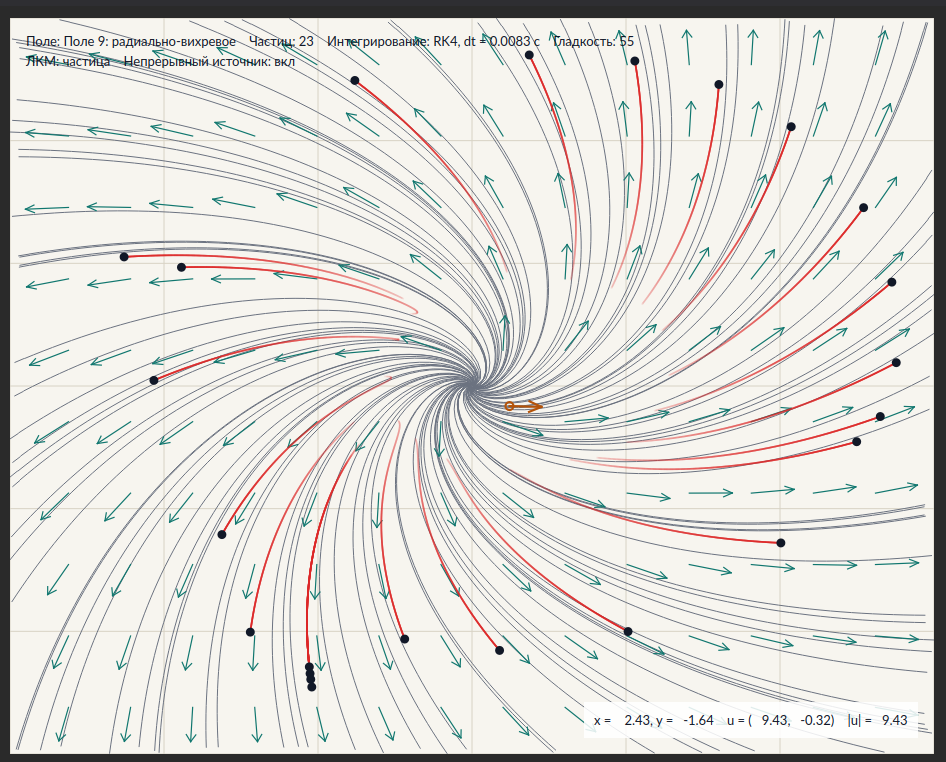
\includegraphics[width=\textwidth]{field9-with-particles-hold-on.png}
\caption{Общий вид программы в режиме интерактивного эксперимента}
\label{fig:overview}
\end{figure}

Отдельный блок интерфейса посвящён описанию поля скорости. Как видно на
рис.~\ref{fig:fieldparams}, пользователь может выбрать один из встроенных
режимов либо, в пользовательском случае, ввести собственные выражения для двух
компонент поля. Отображение краткого текстового описания поля под списком режимов
облегчает восприятие и делает интерфейс пригодным для учебной демонстрации.

\begin{figure}[!htbp]
\centering
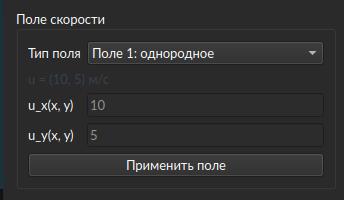
\includegraphics[width=0.55\textwidth]{field-params.png}
\caption{Блок выбора и задания параметров поля скорости}
\label{fig:fieldparams}
\end{figure}

На рис.~\ref{fig:viewparams} показан блок настройки отображения. Переключатели
позволяют независимо включать и отключать различные виды графических объектов,
а ползунок регулирует гладкость линий тока. Это решение оказалось важным на
практике: при одних сценариях удобно видеть лишь стрелки поля, а при других ---
подробную геометрию течения и длинные следы частиц.

\begin{figure}[!htbp]
\centering
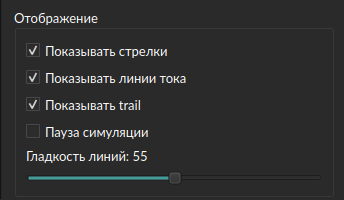
\includegraphics[width=0.56\textwidth]{view-params.png}
\caption{Панель настройки отображения и гладкости линий тока}
\label{fig:viewparams}
\end{figure}

В совокупности рис.~\ref{fig:overview}--\ref{fig:viewparams} показывают, что
интерфейс программы остаётся минималистичным, но при этом покрывает все ключевые
сценарии работы. Такой баланс простоты и функциональности был одной из важных
целей практики.

Новый блок параметров частицы показан на рис.~\ref{fig:particleparams}. В нём
задаются радиус, плотность, начальная скорость по двум координатам и режим
непрерывного источника. Этот блок переводит приложение из демонстрационного
режима в режим серии сопоставимых экспериментов: пользователь может варьировать
не только поле, но и свойства инерционной частицы.

\begin{figure}[!htbp]
\centering
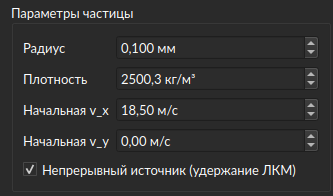
\includegraphics[width=0.56\textwidth]{particle-params.png}
\caption{Панель задания параметров создаваемой частицы и непрерывного источника}
\label{fig:particleparams}
\end{figure}

На рис.~\ref{fig:cursorprobe} показана локальная диагностика под курсором.
Оранжевая стрелка отображает значение поля скорости в выбранной точке, а в углу
окна выводятся координаты и численные значения компонентов вектора. Такая функция
особенно полезна при разборе зон с резким поворотом потока и вблизи центров
вихревого движения.

\begin{figure}[!htbp]
\centering
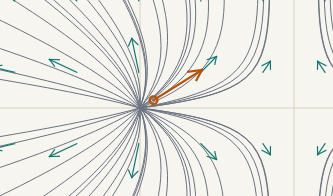
\includegraphics[width=0.42\textwidth]{velocity-vecor-under-cursor.png}
\caption{Локальный вектор скорости под курсором}
\label{fig:cursorprobe}
\end{figure}

\subsection{Примеры экранных форм и численных экспериментов}

Для поля~2 приложение строит существенно более сложную картину, чем для
однородного потока. На рис.~\ref{fig:field2noparticles} показана визуализация
самого поля без частиц. По серым линиям тока видно, что структура течения в правой
части области заметно отличается от поведения слева: траектории изгибаются,
образуя участки с более интенсивной неоднородностью. Стрелки подтверждают, что
направление потока остаётся в целом направленным вправо и вверх, однако модуль и
локальная геометрия меняются от точки к точке.

\begin{figure}[!htbp]
\centering
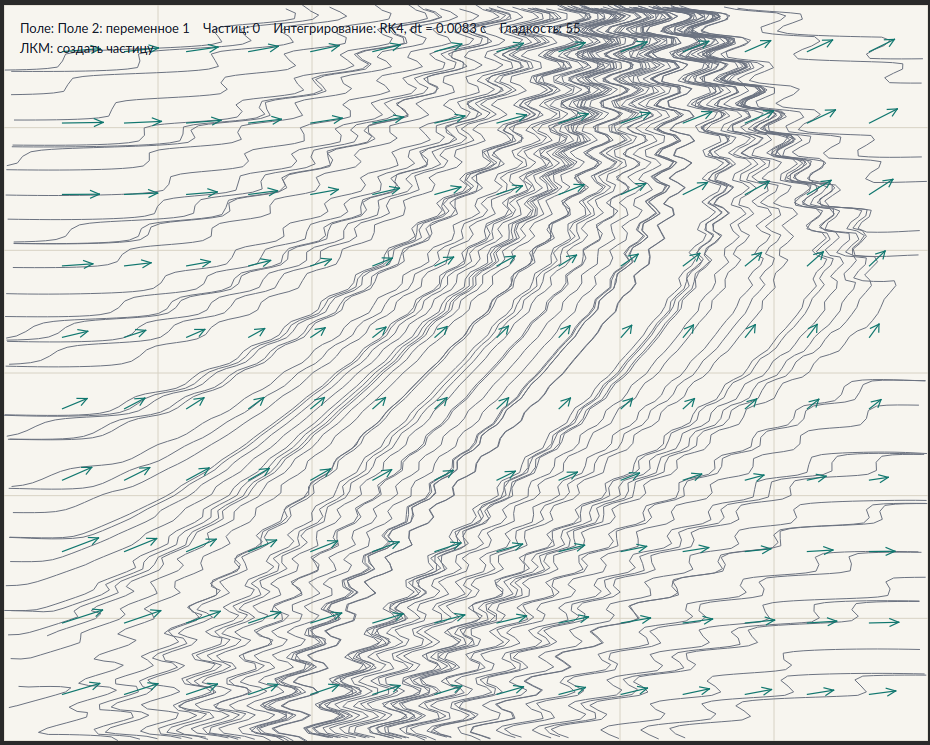
\includegraphics[width=\textwidth]{field2-viewer.png}
\caption{Переменное поле скорости~2 без частиц}
\label{fig:field2noparticles}
\end{figure}

Если в то же поле добавить частицы, как показано на рис.~\ref{fig:field2particles},
становится видно, что реальные траектории не копируют линии тока буквально.
Красные следы сглаживают локальные изменения направления, поскольку частица
обладает собственной скоростью и инерцией. Дополнительное затухание старых
участков следа делает текущую геометрию движения более читаемой и позволяет
быстрее выделить последние изменения траектории.

\begin{figure}[!htbp]
\centering
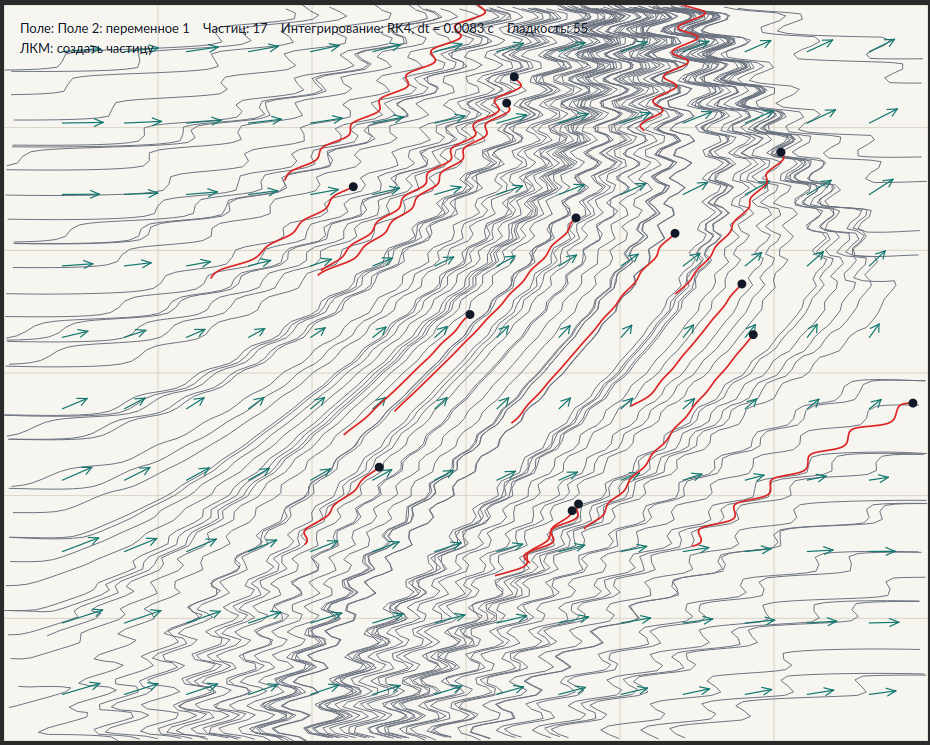
\includegraphics[width=\textwidth]{field2-with-particles-viewer.png}
\caption{Переменное поле скорости~2 с добавленными частицами и их следами}
\label{fig:field2particles}
\end{figure}

Ещё более выразительным является поле с двумя источниками, показанное на
рис.~\ref{fig:field10particles}. Здесь линии тока формируют две конкурирующие
системы выноса, а частицы, помещённые в разные области, реагируют на разные
центры притяжения геометрии потока. В такой конфигурации особенно полезно наличие
стрелок поля: по ним можно сразу увидеть, в какую сторону направлен локальный
вектор скорости и как его модуль меняется при приближении к источникам.

\begin{figure}[!htbp]
\centering
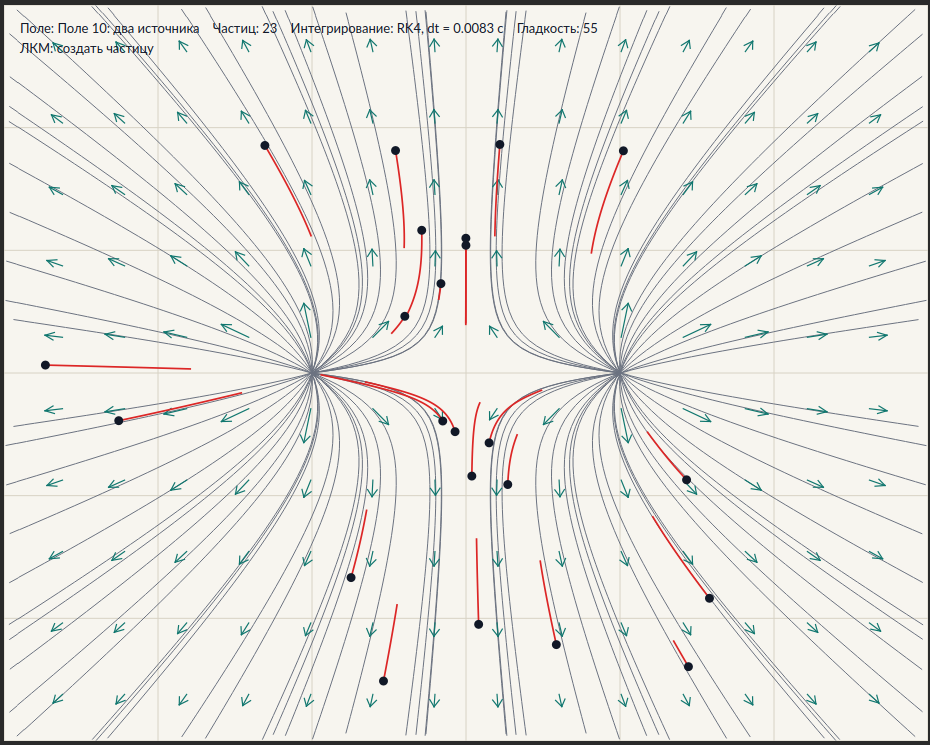
\includegraphics[width=\textwidth]{field10-with-particle-viewer.png}
\caption{Поле с двумя источниками скорости и траектории добавленных частиц}
\label{fig:field10particles}
\end{figure}

На рис.~\ref{fig:field9source} показан режим непрерывного источника в
радиально-вихревом поле. В этом режиме частицы порождаются при удержании левой
кнопки мыши, что позволяет наблюдать не одну отдельную траекторию, а поток
частиц с одинаковыми начальными параметрами. На том же изображении видны
локальная стрелка под курсором и численное значение поля в выбранной точке.

\begin{figure}[!htbp]
\centering
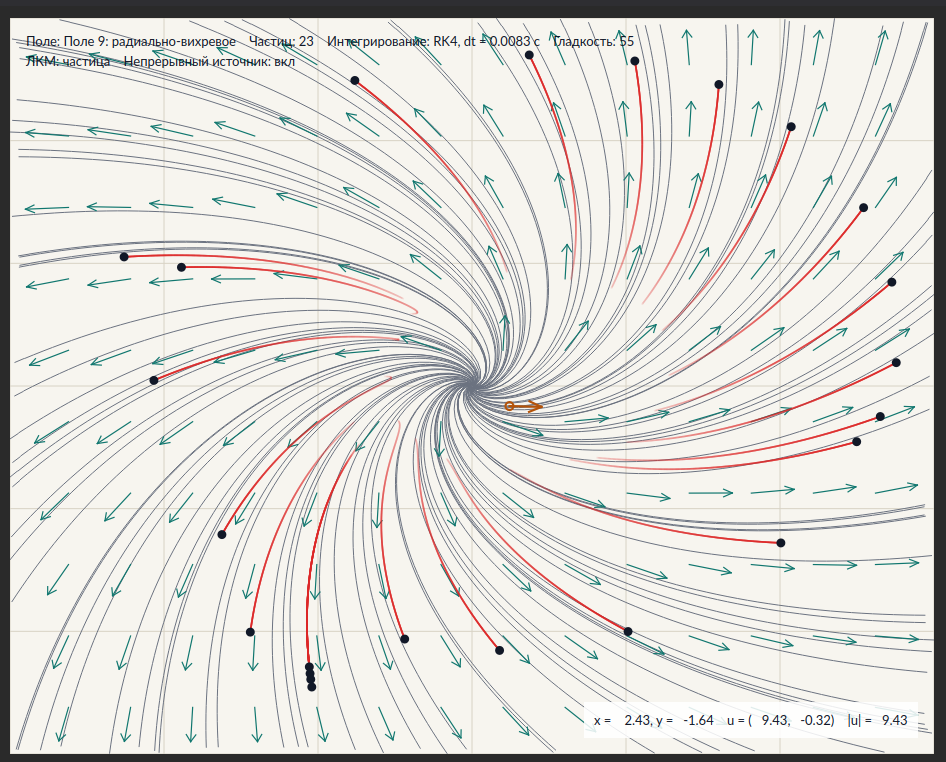
\includegraphics[width=\textwidth]{field9-with-particles-hold-on.png}
\caption{Режим непрерывного источника и локальная диагностика в поле~9}
\label{fig:field9source}
\end{figure}

\subsection{Устойчивость, тестирование и качество визуализации}

В процессе разработки были выполнены последовательные проверки устойчивости
программы. Во-первых, тестировалась корректность вычисления полей скорости при
переключении между встроенными режимами. Во-вторых, проверялась стабильность
численного интегрирования после добавления большого числа частиц в разные области
сцены. В-третьих, оценивалось поведение интерфейса при изменении параметра
гладкости линий тока, поскольку именно этот параметр непосредственно влияет на
объём предварительных вычислений перед отрисовкой.

В ходе тестирования был выявлен важный численный аспект: в некоторых конфигурациях
частица могла выйти в область экстремальных значений координат, что приводило бы
к переполнению отдельных аналитических выражений. Для устранения этой проблемы в
программу были введены проверки на конечность состояния и разумные пределы по
координатам и скоростям. Если состояние частицы перестаёт быть численно надёжным,
она исключается из дальнейшего обновления, не влияя на работу остальной сцены.

Отдельное внимание уделялось качеству линий тока. Первоначально их построение
было более грубым, что визуально проявлялось в ломаной геометрии кривых. После
этого алгоритм был улучшен: увеличено число стартовых точек, уменьшен шаг
интегрирования и добавлено управление детализацией через ползунок в интерфейсе.
В результате пользователь получил возможность самостоятельно выбирать между более
быстрым, но грубым построением и более детализированной визуализацией.

С инженерной точки зрения это важно потому, что приложение ориентировано на
реальное взаимодействие в окне. Каждое улучшение качества должно быть совместимо
с отзывчивостью UI. Практика показала, что выбранная архитектура удерживает этот
баланс: линии тока перестраиваются при изменении параметров, а движение частиц
обновляется в ритме таймера без заметного нарушения плавности.

\subsection{Результаты реализации}

В ходе преддипломной практики была разработана работоспособная интерактивная
программа, демонстрирующая движение частиц в двумерных полях скоростей. Полученное
приложение позволяет наглядно исследовать структуру потока, сравнивать траектории
частиц с линиями тока и быстро тестировать различные конфигурации поля.

На текущем этапе приложение включает полный минимально необходимый набор
функций для интерактивного эксперимента: выбор аналитического поля скорости,
пользовательский ввод формул, отображение стрелок и линий тока, создание частиц
с настраиваемыми параметрами, отображение затухающих следов, непрерывный источник
частиц и локальную диагностику поля под курсором. Тем самым реализован не только
графический интерфейс к уже существующей модели, но и удобный инженерный слой для
качественного анализа поведения частиц в неоднородных течениях.

\newpage
\section*{ЗАКЛЮЧЕНИЕ}
\addcontentsline{toc}{section}{ЗАКЛЮЧЕНИЕ}

В период преддипломной практики была решена задача создания интерактивного
программного средства для визуализации движения частиц в заданных полях скорости.
Разработанное приложение использует математическую модель, основанную на учёте
силы аэродинамического сопротивления, и сохраняет преемственность с ранее
подготовленным дипломным проектом по структуре обозначений, набору полей скорости
и численным методам.

Практическим результатом работы стало настольное приложение, позволяющее в режиме
реального времени строить линии тока, отображать поле скорости стрелками,
создавать частицы с заданными параметрами, подавать их непрерывным источником,
отображать затухающие следы и получать локальные значения поля под курсором.

С инженерной точки зрения основным результатом стала рабочая модульная система,
в которой вычисление поля, динамика частицы, рендер и пользовательский интерфейс
разделены по независимым компонентам. Это позволило совместить физическую
содержательность модели с интерактивной работой в реальном времени и обеспечить
устойчивость приложения при сложных сценариях счёта.

Таким образом, цель преддипломной практики достигнута. Разработано интерактивное
приложение, основанное на содержательной математической модели и пригодное для
демонстрации и качественного анализа движения частиц в двумерных полях скоростей.

\newpage
\begin{thebibliography}{99}
\addcontentsline{toc}{section}{СПИСОК ЛИТЕРАТУРЫ}

\bibitem{Nigmatulin1978}
Нигматулин Р. И. Основы механики гетерогенных сред. --- М.: Наука, 1978. --- 336~с.

\bibitem{SamarskiiGulin}
Самарский А. А., Гулин А. В. Численные методы: учеб. пособие для вузов. ---
М.: Наука. Гл. ред. физ.-мат. лит., 1989. --- 432~с.

\bibitem{Kalitkin}
Калиткин Н. Н. Численные методы: учеб. пособие. --- 2-е изд., испр. ---
СПб.: БХВ-Петербург, 2011. --- 592~с.

\bibitem{LandauLifshitz}
Ландау Л. Д., Лифшиц Е. М. Теоретическая физика: в 10 т. Т. VI:
Гидродинамика. --- 5-е изд., стер. --- М.: ФИЗМАТЛИТ, 2001. --- 736~с.

\bibitem{Loitsyanskii}
Лойцянский Л. Г. Механика жидкости и газа: учебник для вузов. --- 7-е изд.,
испр. --- М.: Дрофа, 2003. --- 840~с.

\bibitem{ProkhorenokDronov}
Прохоренок Н. А., Дронов В. А. Python 3 и PyQt 5. Разработка приложений. ---
2-е изд. --- СПб.: БХВ-Петербург, 2019. --- 832~с.

\bibitem{Qt6}
Документация Qt 6 [Электронный ресурс]. --- URL:
\url{https://doc.qt.io/qt-6/} (дата обращения: 16.05.2026).

\bibitem{Pyside}
Документация PySide6 [Электронный ресурс]. --- URL:
\url{https://doc.qt.io/qtforpython/} (дата обращения: 16.05.2026).

\bibitem{PythonDocs}
Документация языка Python 3 [Электронный ресурс]. --- URL:
\url{https://docs.python.org/3/} (дата обращения: 16.05.2026).
\end{thebibliography}

\end{document}